\begin{figure}[h]        
    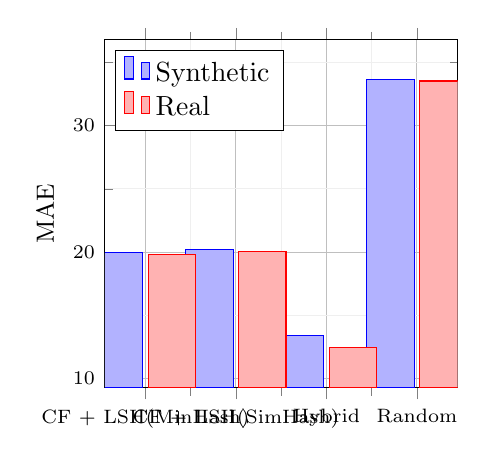
\begin{tikzpicture}
        \begin{axis}[
            enlargelimits=0.15,
            x tick label style={
            /pgf/number format/1000 sep=},
            ylabel={\small{MAE}},
            width = 0.5*\textwidth, 
            height = 6cm,
            legend pos=north west,
            symbolic x coords={CF + LSH(MinHash), CF + LSH(SimHash), Hybrid, Random},
            xtick=data,
            tick label style={font=\scriptsize},
            ybar,
            bar width = .6cm,
            grid = both,
            minor tick num = 1,
            major grid style = {lightgray},
            minor grid style = {lightgray!25},
            legend cell align = {left},
            legend pos = north west
        ]
        
        \addplot coordinates {(CF + LSH(MinHash),19.932730) (CF + LSH(SimHash),20.168860) (Hybrid,13.415692) (Random,33.618878)};
        \addplot coordinates {(CF + LSH(MinHash),19.796775) (CF + LSH(SimHash),20.022409) (Hybrid,12.450330) (Random,33.535856)};
        
        \legend{Synthetic,Real}
        \end{axis}
    \end{tikzpicture}
    
    \caption{\normalfont Average MAE of the different algorithms on the two datasets.}
    \label{fig:mae_histo}
\end{figure}

